\chapter{Operator Splitting Ability}

\modinfo{Solvers}{\Idx{HeatSolve}} 
\modinfo{Tools}{\Idx{ElmerFront}} 
\modinfo{Dimensions}{2D, Steady-state}

\subsection*{Problem description}

An L-shaped structure (see figure~\ref{fg:struct1}) is heated by an internal 
heat source magnitude of which is 1 W/m$^3$. The density of the structure 
material is 1 kg/m$^3$ and its heat conductivity is 1 W/mK. All the 
boundaries $\Gamma_i$ are kept on constant temperature of 0 K. The problem is 
to solve the temperature distribution in the structure.

\begin{figure}
\begin{center}
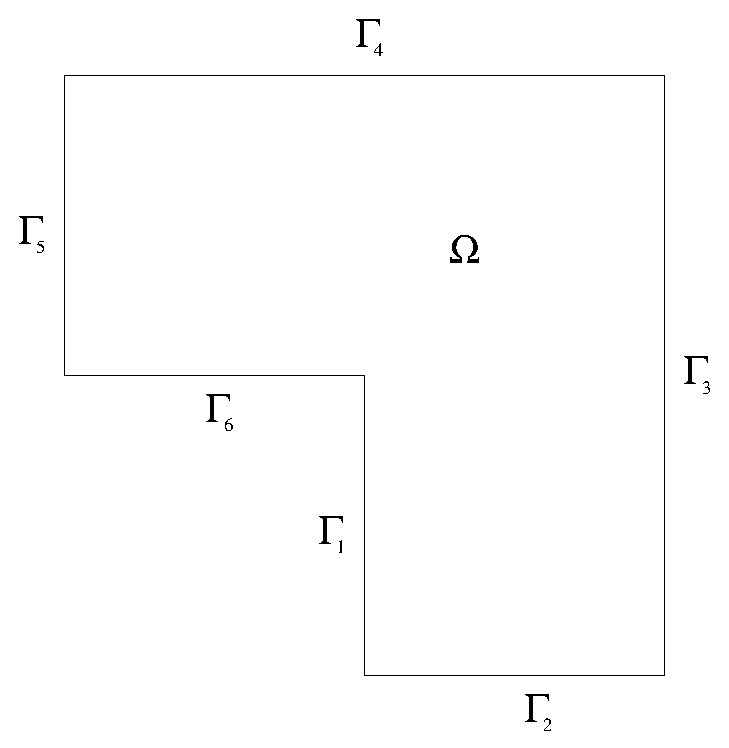
\includegraphics[width=60mm]{Area1}
\caption{L-shaped structure}\label{fg:struct1}
\end{center}
\end{figure}

Mathematically the problem to be solved is
\begin{equation}
\left \{
\begin{array}{cccc}
- \kappa \Delta T &= &f & \mbox{ in } \Omega \\
T&=&0 & \mbox{ on } \Gamma
\end{array}
\right .
\end{equation}
where $\kappa$ is the heat conductivity, $T$  is the temperature 
and $f$ is the heat source. It is assumed that density 
and heat conductivity are constants. 

\subsection*{Solution procedure}

\begin{itemize}
\item Start Elmer in the desired directory with the command
\ttbegin
ElmerFront
\ttend
\item Open the file that contains the geometry of the structure from 
the File menu. Select also the working directory for the model.
\ttbegin
File -> Open cad-file 
  File = TempDist.egf 
  Model name = TempDist 
  Model directory = split_tutorial
\ttend
\item Select the equations to be solved from the Problem menu. In this 
case there is only one equation, the heat equation. Remember to add the 
equation to the equation sets. This connects the equation to the defined 
body. 
\ttbegin
Problem ->\ldots Equations 
  Heat equation 
\ttend
\item Apply the body forces from the Model menu. Give the value for the body 
force (heat source). Remember to add the body forces to the body force 
sets so that they have an effect on $\Omega$ (see figure~\ref{fg:struct1}). 
\ttbegin
Model -> Body forces 
  Heat source = 1
\ttend
\item Define the material properties from the Model menu. Give the values for 
the density and the heat conductivity. Add the defined material properties 
to the material property sets so they become attached to $\Omega$. 
\ttbegin
Model -> Materials 
  Density = 1 
  Heat conductivity = 1
\ttend
\item Define boundary conditions from the Model menu. Give the value of the 
temperature at the boundaries $\Gamma_i$. Add the defined boundary condition 
to boundary condition sets and attach the constraint to all the boundaries 
$\Gamma_i (i=1,\ldots,6)$ of $\Omega$ (see figure~\ref{fg:struct1}). 
\ttbegin
Model -> Boundary conditions 
  Temperature = 0 
\ttend
\item Define mesh for the structure from the Mesh menu. First give name for 
the mesh and then define the element size. Make the mesh by pressing
``Generate mesh'' button. 
\ttbegin
Mesh -> Define mesh 
  Mesh name = Mesh1 
  Model Mesh H [m] = 0.1 
  Generate mesh
\ttend
\item Now to solve the problem select from the Run menu item Solver. This 
starts the solver. 
\ttbegin
Run -> Solver 
\ttend
\item After the solution is done, view the results by selecting from the Run
menu item Postprocessor. 
\ttbegin
Run -> Postprocessor 
\ttend
\item To save the created model, select from the File menu item Save 
model file. 
\ttbegin
File -> Save model file 
\ttend
\item To exit Elmer select from the File menu item Exit. 
\ttbegin
File -> Exit
\ttend
\end{itemize}

\subsection*{Results}

As a result a maximum temperature in the structure is given. For a 
comparison the same problem was solved six times with different 
element sizes. The maximum temperature obtained
by using different meshes is recorded in table~\ref{tb:struct1}.
From the results you can see that the result converges. With a denser mesh 
the result is more accurate, but it takes more calculation time. 

\begin{table}
\caption{Results with different element sizes}
\label{tb:struct1}
\begin{center}
\begin{tabular}{lll} \hline
Model Mesh H [m]  & Elements & $\max (T)$ [K] \\ \hline
0.2 & 186 &  0.14267 \\ 
0.15 & 326 & 0.1462  \\ 
0.1 &  726 & 0.14788 \\
0.05 & 2 792 & 0.1487  \\ 
0.025 & 11 078 & 0.14919  \\ 
0.01  & 69 642 & 0.14935 \\ \hline
\end{tabular}
\end{center}
\end{table}




